\documentclass[a4paper,12pt]{report}
\usepackage[left=2.5cm, right=2cm, top=2cm, bottom=2cm, bindingo ffset=0cm]{geometry}
\usepackage{placeins}
\usepackage{graphicx}
\usepackage{amssymb}
\usepackage[table,xcdraw]{xcolor}
\graphicspath{{C:\Users\User\Desktop\mipt\phys\lab116}}
\DeclareGraphicsExtensions{.pdf,.png,.jpg}
\usepackage[T2A]{fontenc}
\usepackage[utf8]{inputenc}
\usepackage[english,russian]{babel}
\usepackage{amsmath,amsfonts,amssymb,amsthm,mathtools}
\usepackage{wasysym}
\usepackage{wrapfig}
\author{Выполнил Мещеряков Всеволод}
\title{Отчет по лабораторной работе № 1.1.6\\[15pt] «Изучение электронного осциллографа»}
\date{\today}

\begin{document}

\maketitle
	
	\section{\Large Аннотация:}
	\text\par{	Цель работы заключается в исследовании осциллографа, его функций и основных характеристик. Используемые приборы: осциллограф и генератор сигналов.}
	\\
	\text\par{	Лабораторная работа проводится с использованием учебного осциллографа, разработанного на основе осциллографов С1-94 и С1-1.} 
	
	\section{\Large Теоретические сведения: }
	\paragraph{\Large Электронно-лучевая трубка } \text{ }
	\\
	\text\par{	Основной частью электронного осциллятора является электронно-лучевая трубка (см.Рис.\ref{lab116ris1.png). Она представляет собой стеклянную откачанную до высокого вакуума колбу, в которой расположена система катодов и анодов.} 
	
	\begin{figure}[h!]
	\begin{center}
	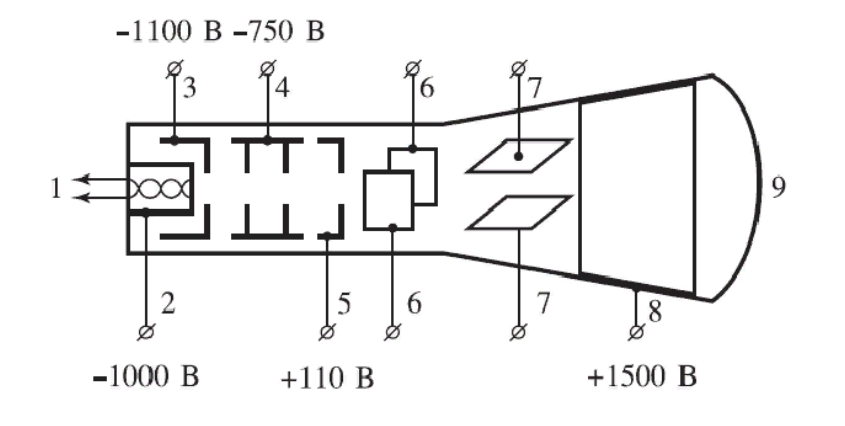
\includegraphics[scale=0.7]{lab116ris1.png} \label{lab116ris1.png}
	\end{center}
	
	\caption{\textit{Электронно-лучевая трубка. 1 - Подогреватель катода, 2 - Катод, 3 - Модулятор, 4 - Фокусирующий анод, 5 - Ускоряющий анод, 6 и 7- Отклоняющие пластины, 8 - Ускоряющий анод, 9 - Экран.}} \label{ris1}
	\end{figure}

	\text\par{Электронный пучок формируется системой из катода с нагревателем, модулятора, фокусирующего и ускоряющего анодов - эта система называется <<электронной пушкой>>. Потенциал фокусирующего анода относительно катода изменяется ручкой <<ФОКУС>> - это определяет размер пятна на экране. Яркость же определяется током электронного луча, который регулируется изменением напряжения на модуляторе ручкой <<ЯРКОСТЬ>>.}
	\\
	\text\par{	На пути к экрану сформированный пучок электронов проходит через два электрических поля отклоняющих пластин 6 и 7. Вертикальные пластины отклоняют пучок в горизонтальном направлении, горизонтальные - в вертикальном. Подавая на пластины соответствующие напряжения, можно <<нарисовать>> электроным лучом на экране некоторую фигуру.}	
	\\
	\text\par{	Рассмотрев движение электронов в эдектрическом поле отклоняющих пластин. Записав кинематические уравнения, геометрические связи и второй закон Ньютона, в итоге получим формулу для смещения луча}
	
	\begin{equation}
	h=\frac{l_1L}{2dU_a} U_y , \label{h}
	\end{equation}
	
	\text\par{которая показывает, что смещение пропорционально отклоняющему напряжению. Из этой же формулы получим чувствительность трубки к напряжению:}
	
	\begin{equation}
	k=\frac{h}{U_y}=\frac{l_1L}{2dU_a} . \label{k}
	\end{equation}

	 \text\par{Эта формула применима и в том случае, когда на отклоняющие пластины подается переменное напряжение, но при условии, что оно мало изменяется за время пролета электрона между пластинами. Характерным интервалом времени, которое определяет скорость изменнеия переменного сигнала, например, может быть период сигнала. Выражение (\ref{h}) определяет координату точки попадания на экран, если частота синусоидального напряжения, подаваемого на отклоняющие пластины, не превышает 0,1 ГГц.}
	 \\	 
	 \text\par{	 Таким образом, смещение луча на экране ЭЛТ можно считать пропорциональным мгновенному значению напряжения на соответствующих отклоняющих пластинах.}
	 
	\paragraph{\Large Развёртка } \text{ }
	\\
	\text\par{	Для получения на экране ЭЛТ <<изображения>> периодического сигнала $U_c(t)$ необходимо выполнение двух условий.}
	\\
	\text\par{ {   } 1. Подаваемое на вертикально отклоняющие пластины напряжение $U_y$ должно линейно зависеть от сигнала $U_c$:}
	
	\begin{equation}		
	U_y(t)=U_{0y}+k_{yu}U_c(t), \label{uy}
	\end{equation}
	
	\text\par{2. Подаваемое на горизонтально отклоняющие пластины напряжение $U_x$ должно линейно зависеть от времени t:}
	
	\begin{equation}
	U_x=U_{0x}+k_{xu}t. \label{ux}
	\end{equation}
	
	\text\par{В (\ref{ux}) и (\ref{uy}) $U_{0x}$ и $U_{0y}$ - напряжения, определяющие расположение графика сигнала по осям oX и oY соответственно, а $k_{yu}$ и $k_{xu}$ - коэффициенты пропорциональности, зависящие от характеристик системы.}
	
	\paragraph{\Large Фигуры Лиссажу} \text{ }
	\\
	\text\par{Фигуры (см. Рис.\ref{lab116ris2.png}), которые описывает луч при сложении с кратными частотами, называются фигурами Лиссажу. При небольшом нарушении кратности частот форма фигур медленно меняется, а при большом - размывается.}
	
	\begin{equation}
	\frac{x^2}{A^2}+\frac{y^2}{B^2}-2\frac{xy}{AB}\cos(\varphi_2-\varphi_1)=\sin^2(\varphi_2-\varphi_1),\label{traek}
	\end{equation}
	\[x=A\cos(2\pi ft+\varphi_1),\]
	\[y=B\cos(2\pi ft+\varphi_2),\] 
	\[A=k_xU_a,\]
	\[B=k_yU_b.\]
	
	\begin{figure}[h!]
	\begin{center}
	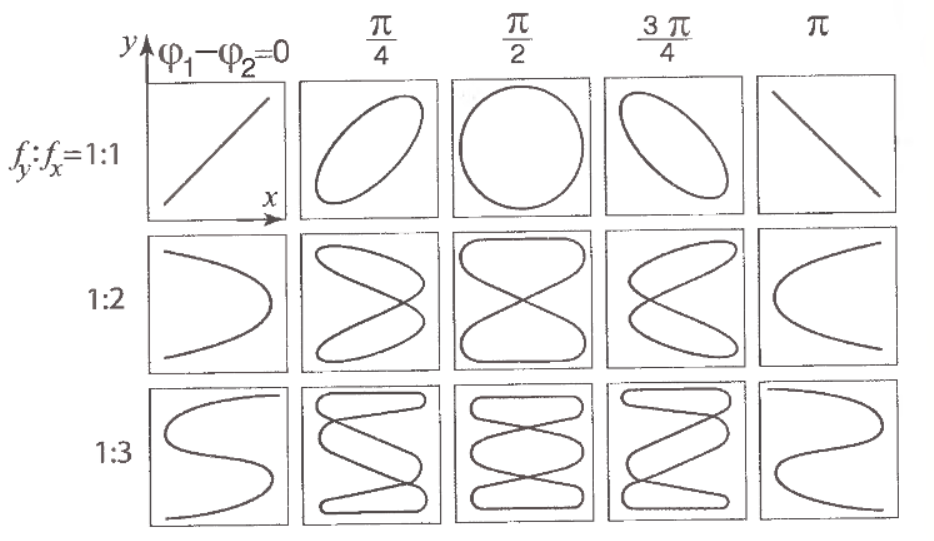
\includegraphics[scale=0.5]{lab116ris2.png}
	\end{center}
	\caption{\textit{Фигуры Лиссажу для колебаний одинаковой амплитуды.}} \label{lab116ris2.png}
	\end{figure}
	
	\section{\Large Измерения, анализ их результатов}
	
	\paragraph{Задание 1. Измерение амплитуды синусоидального сигнала. }
	
	\text\par{ \\ Настроим осциллограф согласно рекомендациям и приступим к измерению.}
	\\
	\text\par{ { }	 Минимальное значение:}
	
	\begin{center}
	
	$volt/divison=5\times10^{-2}$ Вольт, \\ $U_{min}=12 \times 10^{-3} \pm 0,2 \times 10^{-3}$ Вольт.
	
	\end{center}
	
	\text\par{Максимальное значение:}
	
	\begin{center}
	
	$volt/divison=5$ Вольт, \\ $U_{max}=21 \pm 0,5$ Вольт.
	
	\end{center}
	
	\text\par{Тогда $\beta$[Дб] - отношение максимального значения к минимальному:}
	
	\begin{center}
	
	$\beta=20\log{\frac{U_{max}}{U_{min}}}=65$ Дб.
	
	\end{center}
	
	\text\par{Децибелл - логарифмическая единица ослабления или усиления сигнала. }	
	

	\paragraph{Задание 2. Измерение амплитудно-частотной характеристики осциллографа.}

	\text\par{Амплитудно-частотной характеристикой (АЧХ) измерительного прибора называют зависимость амплитуды измеряемого сигнала от частоты сигнала, подаваемого на вход. Проведем измерения АЧХ и занесем их в таблицу 1.}
	
	\begin{figure}[h!]
	\begin{center}
	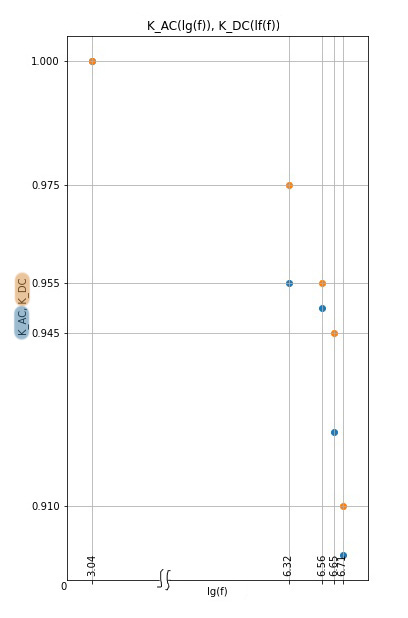
\includegraphics[scale=1]{lab116ris3.jpg}
	\caption{\textit{График АЧХ усилителей каналов.}}
	\end{center}
	\end{figure}
	
	\begin{center}
	\begin{table}[h]
\begin{tabular}{|c|c|c|c|c|c|}
\hline
\text{f}                     & \text{$1,1\times10^3$} & \text{$2,1\times10^6$} & \text{$3,64\times10^6$} & \text{$4,5\times10^6$} & \text{$5,1\times10^6$} \\ \hline
\text{$\lg{f}$}              & \text{3,04}            & \text{6,32}            & \text{6,56}             & \text{6,65}            & \text{6,71}            \\ \hline
\text{$2A_{y}$, деления}     & \text{4,1}             & \text{3,8}             & \text{3,8}              & \text{3,7}             & \text{3,6}             \\ \hline
\text{$K_{AC}=U_{AC}/U_{0}$} & \text{1}               & \text{0,95}            & \text{0,95}             & \text{0,925}           & \text{0,9}             \\ \hline
\text{$2A_{DC}$, деления}    & \text{4}               & \text{3,9}             & \text{3,8}              & \text{3,8}             & \text{3,9}             \\ \hline
\text{$K_{DC}=U_{DC}/U_{0}$} & \text{1}               & \text{0,975}           & \text{0,95}             & \text{0,95}            & \text{0,9}             \\ \hline
\end{tabular}
\caption{\textit{АЧХ усилителей каналов.}}
\end{table}
\end{center}

	\paragraph{Задание 3. Измерение разности фазово-частотных характеристик каналов осциллографа.} \text{ }
	\\
	\text\par{Проведем измерения разности фаз, возникающей при подаче одного и того же сигнала на разные каналы осциллографа - фазово-частотную характеристику в зависимости от частоты сигнала. Результаты измерений смотреть на таблице 2 и их графическую интерпретацию рисунке 3.}
	
\text\par{Из графика становится ясно, что осциллограф может пользоваться для измерения разности частот, не превосходящих $10^5$ Гц.}

\section{Обсуждение результатов и выводы.}

\text\par{В работе исследовано устройство и принципы работы осциллографа. Также найдены частоты, работа при которых допустима. Были исследованы амплитудно-частотные и фазово-частотные характеристики осциллографа GOS-620.}

\begin{table}[h!]
\begin{tabular}{|c|c|c|c|c|c|c|c|}
\hline
Величина\textbackslash N эксперимента & 1  & 2   & 3    & 4     & 5           & 6           & 7           \\ \hline
f, Гц                                   & 10 & $10^2$ & $10^3$ & $10^4$ & $10^5$      & $10^6$     & $5\times10^6$     \\ \hline
$\log{f}$                             & 1  & 2   & 3    & 4     & 5           & 6           & 6,7 \\ \hline
2$y_0$, дел                           & 0  & 0   & 0    & 0     & 0,1         & 1           & 1           \\ \hline
2$A_y$, дел                           & 2  & 2   & 2    & 2     & 2           & 2           & 2           \\ \hline
$\arcsin{y_0/A_y}$ , рад                   & 0  & 0   & 0    & 0     & 0,05 & 0,52 & 0,52 \\ \hline
$\Delta\varphi$ , рад                    & 0  & 0   & 0    & 0     & 0,05 & 0,52 & 0,52 \\ \hline
\end{tabular}
\caption{\textit{Снятые данные для вычисления зависимости $\Delta\varphi$ от $\log{f}$.}}
\end{table}	

\begin{figure}[h]
	\begin{center}
	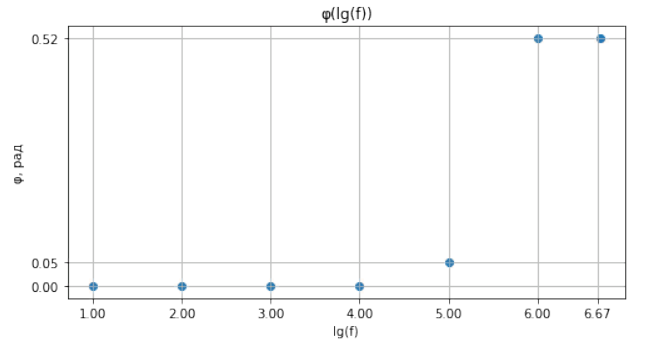
\includegraphics[scale=1]{lab116ris4.png}
	\caption{\textit{Зависимость разности фаз $\Delta\varphi$ от десятичного логарифма частоты $\log{f}$.}}
	\end{center}
	\end{figure}
	

\end{document}
